% Options for packages loaded elsewhere
\PassOptionsToPackage{unicode}{hyperref}
\PassOptionsToPackage{hyphens}{url}
%
\documentclass[
]{article}
\usepackage{lmodern}
\usepackage{amssymb,amsmath}
\usepackage{ifxetex,ifluatex}
\ifnum 0\ifxetex 1\fi\ifluatex 1\fi=0 % if pdftex
  \usepackage[T1]{fontenc}
  \usepackage[utf8]{inputenc}
  \usepackage{textcomp} % provide euro and other symbols
\else % if luatex or xetex
  \usepackage{unicode-math}
  \defaultfontfeatures{Scale=MatchLowercase}
  \defaultfontfeatures[\rmfamily]{Ligatures=TeX,Scale=1}
\fi
% Use upquote if available, for straight quotes in verbatim environments
\IfFileExists{upquote.sty}{\usepackage{upquote}}{}
\IfFileExists{microtype.sty}{% use microtype if available
  \usepackage[]{microtype}
  \UseMicrotypeSet[protrusion]{basicmath} % disable protrusion for tt fonts
}{}
\makeatletter
\@ifundefined{KOMAClassName}{% if non-KOMA class
  \IfFileExists{parskip.sty}{%
    \usepackage{parskip}
  }{% else
    \setlength{\parindent}{0pt}
    \setlength{\parskip}{6pt plus 2pt minus 1pt}}
}{% if KOMA class
  \KOMAoptions{parskip=half}}
\makeatother
\usepackage{xcolor}
\IfFileExists{xurl.sty}{\usepackage{xurl}}{} % add URL line breaks if available
\IfFileExists{bookmark.sty}{\usepackage{bookmark}}{\usepackage{hyperref}}
\hypersetup{
  pdftitle={Nudging for less kludges: focusing on PMD alerts as possible kludges: open, fixed or new?},
  pdfauthor={Bruno Crotman},
  hidelinks,
  pdfcreator={LaTeX via pandoc}}
\urlstyle{same} % disable monospaced font for URLs
\usepackage[margin=1in]{geometry}
\usepackage{color}
\usepackage{fancyvrb}
\newcommand{\VerbBar}{|}
\newcommand{\VERB}{\Verb[commandchars=\\\{\}]}
\DefineVerbatimEnvironment{Highlighting}{Verbatim}{commandchars=\\\{\}}
% Add ',fontsize=\small' for more characters per line
\usepackage{framed}
\definecolor{shadecolor}{RGB}{248,248,248}
\newenvironment{Shaded}{\begin{snugshade}}{\end{snugshade}}
\newcommand{\AlertTok}[1]{\textcolor[rgb]{0.94,0.16,0.16}{#1}}
\newcommand{\AnnotationTok}[1]{\textcolor[rgb]{0.56,0.35,0.01}{\textbf{\textit{#1}}}}
\newcommand{\AttributeTok}[1]{\textcolor[rgb]{0.77,0.63,0.00}{#1}}
\newcommand{\BaseNTok}[1]{\textcolor[rgb]{0.00,0.00,0.81}{#1}}
\newcommand{\BuiltInTok}[1]{#1}
\newcommand{\CharTok}[1]{\textcolor[rgb]{0.31,0.60,0.02}{#1}}
\newcommand{\CommentTok}[1]{\textcolor[rgb]{0.56,0.35,0.01}{\textit{#1}}}
\newcommand{\CommentVarTok}[1]{\textcolor[rgb]{0.56,0.35,0.01}{\textbf{\textit{#1}}}}
\newcommand{\ConstantTok}[1]{\textcolor[rgb]{0.00,0.00,0.00}{#1}}
\newcommand{\ControlFlowTok}[1]{\textcolor[rgb]{0.13,0.29,0.53}{\textbf{#1}}}
\newcommand{\DataTypeTok}[1]{\textcolor[rgb]{0.13,0.29,0.53}{#1}}
\newcommand{\DecValTok}[1]{\textcolor[rgb]{0.00,0.00,0.81}{#1}}
\newcommand{\DocumentationTok}[1]{\textcolor[rgb]{0.56,0.35,0.01}{\textbf{\textit{#1}}}}
\newcommand{\ErrorTok}[1]{\textcolor[rgb]{0.64,0.00,0.00}{\textbf{#1}}}
\newcommand{\ExtensionTok}[1]{#1}
\newcommand{\FloatTok}[1]{\textcolor[rgb]{0.00,0.00,0.81}{#1}}
\newcommand{\FunctionTok}[1]{\textcolor[rgb]{0.00,0.00,0.00}{#1}}
\newcommand{\ImportTok}[1]{#1}
\newcommand{\InformationTok}[1]{\textcolor[rgb]{0.56,0.35,0.01}{\textbf{\textit{#1}}}}
\newcommand{\KeywordTok}[1]{\textcolor[rgb]{0.13,0.29,0.53}{\textbf{#1}}}
\newcommand{\NormalTok}[1]{#1}
\newcommand{\OperatorTok}[1]{\textcolor[rgb]{0.81,0.36,0.00}{\textbf{#1}}}
\newcommand{\OtherTok}[1]{\textcolor[rgb]{0.56,0.35,0.01}{#1}}
\newcommand{\PreprocessorTok}[1]{\textcolor[rgb]{0.56,0.35,0.01}{\textit{#1}}}
\newcommand{\RegionMarkerTok}[1]{#1}
\newcommand{\SpecialCharTok}[1]{\textcolor[rgb]{0.00,0.00,0.00}{#1}}
\newcommand{\SpecialStringTok}[1]{\textcolor[rgb]{0.31,0.60,0.02}{#1}}
\newcommand{\StringTok}[1]{\textcolor[rgb]{0.31,0.60,0.02}{#1}}
\newcommand{\VariableTok}[1]{\textcolor[rgb]{0.00,0.00,0.00}{#1}}
\newcommand{\VerbatimStringTok}[1]{\textcolor[rgb]{0.31,0.60,0.02}{#1}}
\newcommand{\WarningTok}[1]{\textcolor[rgb]{0.56,0.35,0.01}{\textbf{\textit{#1}}}}
\usepackage{graphicx}
\makeatletter
\def\maxwidth{\ifdim\Gin@nat@width>\linewidth\linewidth\else\Gin@nat@width\fi}
\def\maxheight{\ifdim\Gin@nat@height>\textheight\textheight\else\Gin@nat@height\fi}
\makeatother
% Scale images if necessary, so that they will not overflow the page
% margins by default, and it is still possible to overwrite the defaults
% using explicit options in \includegraphics[width, height, ...]{}
\setkeys{Gin}{width=\maxwidth,height=\maxheight,keepaspectratio}
% Set default figure placement to htbp
\makeatletter
\def\fps@figure{htbp}
\makeatother
\setlength{\emergencystretch}{3em} % prevent overfull lines
\providecommand{\tightlist}{%
  \setlength{\itemsep}{0pt}\setlength{\parskip}{0pt}}
\setcounter{secnumdepth}{5}
\usepackage{lscape}
\usepackage{amsmath}
\usepackage{smartdiagram}
\usesmartdiagramlibrary{additions}
\newcommand{\blandscape}{\begin{landscape}}
\newcommand{\elandscape}{\end{landscape}}
\definecolor{darkred}{RGB}{150, 40, 40}
\definecolor{darkgreen}{RGB}{30, 120, 30}
\definecolor{darkorange}{RGB}{40, 40, 160}
\newcommand{\comentario}[1]{}
\usepackage{booktabs}
\usepackage{longtable}
\usepackage{array}
\usepackage{multirow}
\usepackage{wrapfig}
\usepackage{float}
\usepackage{colortbl}
\usepackage{pdflscape}
\usepackage{tabu}
\usepackage{threeparttable}
\usepackage{threeparttablex}
\usepackage[normalem]{ulem}
\usepackage{makecell}
\usepackage{xcolor}
\newlength{\cslhangindent}
\setlength{\cslhangindent}{1.5em}
\newenvironment{cslreferences}%
  {\setlength{\parindent}{0pt}%
  \everypar{\setlength{\hangindent}{\cslhangindent}}\ignorespaces}%
  {\par}

\title{Nudging for less kludges: focusing on PMD alerts as possible
kludges: open, fixed or new?}
\author{Bruno Crotman}
\date{}

\begin{document}
\maketitle

{
\setcounter{tocdepth}{2}
\tableofcontents
}
\small

\normalsize

\section{Introduction}\label{intro}

This document is part of a research project about software degradation
caused by careless developers' behavior and about strategies to deal
with such undesired behavior. These strategies will possibly be inspired
by concepts from game theory.

We assume that software degradation can be measured by the number and
the types of \textit{kludges} made by software developers in the code. A
kludge is code that

\begin{enumerate}
\def\labelenumi{\arabic{enumi}.}
\tightlist
\item
  Partially fixes a bug or partially implements a feature.
\end{enumerate}

\setlength{\parindent}{1.0cm}
\hangindent=1.0cm

The term partial can be understood as in \textit{partial functions}. A
partial function is undefined for some elements in the formal domain.
For instance, the square root function restricted to the integers:
\(f(25)\) is defined, but \(f(26)\) is undefined. In terms of features,
we can think about a developer calculating the point on which two lines
cross and neglecting the case of parallel lines;

\begin{enumerate}
\setcounter{enumi}{1}
\tightlist
\item
  The developer knows that the code is only a partial solution, with
  high probability.~\footnote{We need to study technical debt papers
  to enrich the conceptual background.}
\end{enumerate}

This project aims to study how software projects evolve in terms of
number and kinds of kludges. So far, we are trying to identify kludges
by looking at alerts generated by the PMD source code analyzer. PMD is a
static source code analyzer that is commonly used to find potential
programming flaws. PMD is a good choice for a researcher to analyze bad
practices, because it supports multiple languages and it is very
flexible. It allows the researcher to provide his own rules for finding
interesting patterns in a source code in Java or other languages. The
planned steps for this research project are:

\begin{itemize}
\item
  Confirm the assumption that the frequency of PMD alerts is an accurate
  measure of the prevalence of kludges;
  
\item
  Confirm the assumption that kludges harm software development;

\item
  Confirm the assumption that there is a game in which, in Nash
  equilibrium, a developer chooses a strategy in which he gets personal
  benefits while causing harm to the project, by making kludges;

\item
  If all these assumptions are true, use mechanism design to devise how
  we can change the environment in a way that developers do not choose
  to make so many kludges, increasing project quality in the long run;

\item
  Implement this mechanism building a plugin for a prominent CI tool,
  such as Travis, Jenkins or GitLab.
\end{itemize}

In this document, we evaluate PMD Source Code Alerts as proxies for
kludges. In section \ref{pmd}, we present PMD Source Code Analyzer and
show how we use the tool to generate alerts that are possible kludges.
We use this tool, also, to create a simplified AST that will help us in
the algorithm that infers how many new alerts were created, how many
were fixed and how many remain open in a transition from an old version
to a new version. This algorithm is described in Section \ref{alg}. In
Section \ref{results}, we compare the creation of new alerts with the
insertion of Self Admitted Technical Debt (SATD) comments.

% ========================================================= % 
% PMD SOURCE CODE ANALYZER % 
%=========================================================

\section{The PMD Source Code Analyzer}\label{pmd}

We use PMD to list the alerts that represent \textit{possible kludges}
in a source code. PMD receives a source code as input and generates a
list of bad programming practices contained in the code, i.e., the
alerts.

PMD traverses the AST of a source code searching for violations of rules
which are configured by the user. PMD comes with a default rule set for
the Java programming language. The default rule set finds common
programming flaws such as unused variables, empty catch blocks,
unnecessary object creation, and so forth. It is possible to configure a
different set of rules by creating a custom XML file. Below, we can see
a simple code and the alerts that were generated by the default rule
set. In this example, PMD generates two alerts of the type
ControlStatementBraces (CSB), in lines 11 and 20. This alert means that
there are no braces in a statement that is inside a control statement.

\small

\normalsize

\newpage

\small

\begin{Shaded}
\begin{Highlighting}[]
\CommentTok{/*  1{-}   */}\KeywordTok{package}\ImportTok{ pack\_x;}
\CommentTok{/*  2{-}   */}  
\CommentTok{/*  3{-}   */}\KeywordTok{import}\ImportTok{ importX.function;}
\CommentTok{/*  4{-}   */}
\CommentTok{/*  5{-}   */}\KeywordTok{class}\NormalTok{ ClassX }\KeywordTok{extends}\NormalTok{ ClassY }\KeywordTok{implements}\NormalTok{ InterfX \{}
\CommentTok{/*  6{-}   */}    \KeywordTok{private} \DataTypeTok{long}\NormalTok{ fieldX;}
\CommentTok{/*  7{-}   */}    
\CommentTok{/*  8{-}   */}    \FunctionTok{ClassX}\NormalTok{(}\DataTypeTok{int}\NormalTok{ paramX, }\DataTypeTok{double}\NormalTok{ paramY) \{}
\CommentTok{/*  9{-}   */}        \DataTypeTok{int}\NormalTok{ varX = }\FunctionTok{function}\NormalTok{(paramX, paramY);}
\CommentTok{/* 10{-}   */}        \KeywordTok{if}\NormalTok{ (varX == }\DecValTok{0}\NormalTok{)}
\CommentTok{/* 11{-}CSB*/}            \KeywordTok{this}\NormalTok{.}\FunctionTok{fieldX}\NormalTok{ = }\DecValTok{1}\NormalTok{;}
\CommentTok{/* 12{-}   */}        \KeywordTok{else}\NormalTok{\{}
\CommentTok{/* 13{-}   */}            \KeywordTok{this}\NormalTok{.}\FunctionTok{fieldX}\NormalTok{ = }\DecValTok{0}\NormalTok{;}
\CommentTok{/* 14{-}   */}\NormalTok{     \}}
\CommentTok{/* 15{-}   */}\NormalTok{    \}}
\CommentTok{/* 16{-}   */}    \AttributeTok{@Override}
\CommentTok{/* 17{-}   */}    \KeywordTok{public} \DataTypeTok{int} \FunctionTok{methodX}\NormalTok{(}\DataTypeTok{int}\NormalTok{ paramW, }\BuiltInTok{Boolean}\NormalTok{ paramZ)}
\CommentTok{/* 18{-}   */}\NormalTok{    \{}
\CommentTok{/* 19{-}   */}        \KeywordTok{if}\NormalTok{ (paramZ)}
\CommentTok{/* 20{-}CSB*/}\NormalTok{            fieldX = paramW;}
\CommentTok{/* 21{-}   */}        \KeywordTok{else}\NormalTok{\{}
\CommentTok{/* 22{-}   */}\NormalTok{            fieldX = }\DecValTok{0}\NormalTok{;}
\CommentTok{/* 23{-}   */}\NormalTok{     \}}
\CommentTok{/* 24{-}   */}        \KeywordTok{return}\NormalTok{ paramW + }\KeywordTok{this}\NormalTok{.}\FunctionTok{fieldX}\NormalTok{;}
\CommentTok{/* 25{-}   */}\NormalTok{     \}}
\CommentTok{/* 26{-}   */}\NormalTok{\}  }


\NormalTok{CSB: ControlStatementBraces}
\end{Highlighting}
\end{Shaded}

\normalsize

\subsection{Using PMD to capture the history of alerts}\label{history}

To evaluate how the number of alerts evolved throughout the history of a
software project, we must be able to analyze a pair of different
versions of a source code (an old and a new version) and categorise each
alert contained in the code as either \textbf{new}, \textbf{fixed} or
\textbf{open}.

We define a PMD alert generated for the old version as either
\textbf{open} or \textbf{fixed} in the new version. An \textbf{open}
alert remains in the new version of the code. A \textbf{fixed} alert
does not exist in the new version.

A PMD alert generated for the new version is either \textbf{open} or
\textbf{new}. An \textbf{open} alert indicates that the same alert was
identified in the old version of the source code. A \textbf{new} alert
implies that the same alert cannot be identified in the old version.

The intersection between \textbf{fixed} alerts, \textbf{new} alerts and
\textbf{open} alerts is empty. The alerts identified as \textbf{open}
are equivalent in both new and old versions. To decide whether an alert
is \textbf{open}, \textbf{fixed} or \textbf{new}, one has to identify if
this alert in the old version is equivalent to its occurrence in the new
version. This document describes an algorithm to make this
classification.

\subsection{Using PMD to generate an simplified Abstract Syntax Tree }\label{ast}

To classify alerts as \textbf{new}, \textbf{open} and \textbf{fixed}, we
could match the lines of the old version to the lines of the new version
of a source code using a diff functionality. Diff is useful, but not
sufficient. Frequently, the source code changes are more complex than
the ones we could address by using only diff. An alert \(o\) in the old
version could be essentially the same as the alert \(n\) contained in
the new version, but the piece of code where \(o\) resides could be
moved in a way that it is impossible to match \(o\) to \(n\) only using
information from Diff. Section \ref{alg} presents and algorithm that
uses extra information from a simplified AST created using PMD.

PMD traverses the source code by visiting many different kinds of
elements. We do not use all the types of nodes recognized by PMD to
generate the simplified AST because there are many kinds of nodes that
are not needed in the current heuristic that classify the alerts, as
described in Section \ref{heuristic}. If we used all the kinds of nodes,
we would end up with a tree that would not add value to our analysis but
would add complexity to our algorithm. The kinds of elements that were
selected are listed below:

\begin{itemize}


\item \textbf{Block}: a block of statements enclosed by braces;

\item \textbf{ClassOrInterfaceBody}: the body of an interface or a class, excluding the declaration;

\item \textbf{CompilationUnit}: the root of an AST tree;

\item \textbf{Method}: a method, including body and declaration;

\item \textbf{Constructor}: a constructor, including body and declaration;

\item \textbf{Statement}: any statement, like an if statement or an assignment;

\end{itemize}

PMD is prepared to receive an optional XML file, along with the source
generated by PMD. The default XML generates alerts when it finds common
bad practices, but to create the simplified AST we use an XML file with
instructions to generate all the nodes of the kinds we listed above. PMD
output lists these nodes and the location of these nodes in the source
code as shown in Table \ref{tab_nodes}.

\small

\begin{table}[!h]

\caption{\label{tab:unnamed-chunk-2}Output from PMD when creating a simplified AST\label{tab_nodes}}
\centering
\begin{tabular}[t]{l|r|r|r|r}
\hline
Kind of node & Begin line & Begin column & End line & End column\\
\hline
\rowcolor{gray!6}  compilation\_unit & 1 & 1 & 26 & 3\\
\hline
class\_or\_interface\_body & 5 & 48 & 26 & 1\\
\hline
\rowcolor{gray!6}  method & 17 & 12 & 25 & 6\\
\hline
block & 18 & 5 & 25 & 6\\
\hline
\rowcolor{gray!6}  constructor\_declaration & 8 & 5 & 15 & 5\\
\hline
statement & 10 & 9 & 14 & 17\\
\hline
\rowcolor{gray!6}  statement & 19 & 9 & 23 & 17\\
\hline
block & 12 & 13 & 14 & 17\\
\hline
\rowcolor{gray!6}  statement & 12 & 13 & 14 & 17\\
\hline
block & 21 & 13 & 23 & 17\\
\hline
\rowcolor{gray!6}  statement & 21 & 13 & 23 & 17\\
\hline
statement & 11 & 13 & 11 & 28\\
\hline
\rowcolor{gray!6}  statement & 13 & 13 & 13 & 28\\
\hline
statement & 20 & 13 & 20 & 28\\
\hline
\rowcolor{gray!6}  statement & 22 & 13 & 22 & 23\\
\hline
statement & 24 & 9 & 24 & 36\\
\hline
\end{tabular}
\end{table}

\normalsize

Looking at Table \ref{tab_nodes}, we see that there is information about
the location of the nodes, in terms of lines and columns. We can infer
which nodes are contained in other nodes, because we can compare the
begin and end lines and the begin and end columns and we know that if a
node A is inside the contents of a node B (within its range of lines of
code), A is descendant of B in the AST. But we cannot see if the node A
is a child or a grandchild of B (or a grand-grand-child\ldots). We
follow three steps to recreate the AST:

\begin{enumerate}
\item
  Link each node \(a\) to the set of nodes \(X\) that are fully
  contained between the begin line / begin column and end line / end
  column of node \(a\). We can construct a directed graph in which
  the elements are the nodes and the links described are the edges. This
  is not a tree yet, because each node will have edges directed to all
  its descendants and not only its children in the AST;

\item
  Sort the nodes in the decreasing order of its number of children. The
  objective is to establish that, in a search through this graph, the
  first child chosen will be the one that is a child in the AST, and not
  only a descendant;

\item
  Proceed a deep-first search starting from the compilation unit node.
\end{enumerate}

% ========================================================= % 
% RESEARCH QUESTIONS % 
%=========================================================

\section{Research questions}
\label{as_whole}

\noindent
\textbf{RQ: Is the frequency of PMD Alerts an accurate measure of the prevalence of kludges?}
\label{PMD_Kludge}

In a given transition between an old version and a new version we want
to identify if there was an intense introduction of PMD alerts. This
evidence of possible kludge introduction must be normalized by the size
of the change in source code between the two versions. We do this by
following this formula:

\[ \frac{\#NewAlerts - \#FixedAlerts}{Change}    \]

where

\[Change = \#NewAlerts + \#FixedAlerts\]

With these version transition measured in terms of inclusion of PMD
alerts, we can correlate these events with some other evidence of
kludge. In Section \ref{results}, we calculate this correlation using
\textit{Self-Admitted Technical Debt} (SATD) comments.

\vspace{16px}

\noindent \textbf{RQ: Do kludges harm software development?}
\label{kludge_harm}

We need some way to measure degradation after a heavy introduction of
kludges. A drop in the popularity may not be a proper evidence. The
increment in the number of issues and bug fixed nor necessarily
represent a degradation. Churn could be used here.

% ========================================================= 
% ALGORITHMS \% 
%%=========================================================

\section{An algorithm to classify alerts}
\label{alg}

This section discusses the algorithm to classify alerts as open, fixed,
or new. The algorithm uses the simplified AST described in Section
\ref{ast} to create features that help to infer if two alerts in
different versions must be considered the same. We use the term
\textit{feature} as it is used in the field of statistical learning
(Kuhn and Johnson, 2019). In this field, the variables that are used to
predict the outcome of an event are called \emph{independent variables},
\emph{predictors}, or \emph{features}.

The term \emph{feature} is used more appropriately if referring to a
variable that is a composite one or more variables or the result of a
treatment upon raw data. Given a pair of alerts, one from the old
version and one from the new version, we use the mapping between the
lines of the old and the new version and their AST as raw data to create
the features that will be used to infer if if they are the same alert.
At the moment, we use a heuristic to infer if the pair of alerts is the
same, as described in Section \ref{heuristic}. Figure \ref{fig:diag}
shows the steps of the algorithm we are describing.

\begin{figure}
  \centering
  \resizebox{1.0\textwidth}{!}{%
  \smartdiagram[sequence diagram]{Get alerts for each version, Create AST for each version, Map new lines to old lines, Calculate features for each pair of alert, Decide if the alerts are the same, Classify alerts}
  }
  \caption{Steps of the algorithm to classify alerts}\label{fig:diag}
\end{figure}

\subsection{An illustrative example}\label{source_used}

Hereafter, we consider the old and new version of an example of source
code presented below. In the new version, the alert generated in the
line 11 of the old version was fixed, but another remained on the new
version. So we expect one alert \textbf{Fixed} in the old version, one
alert \textbf{Open} in the old version, and the same \textbf{Open} alert
in the new version.

\vspace{12px}
\scriptsize
\begin{Shaded}
\begin{Highlighting}[]
\CommentTok{/*  1{-}   */}\KeywordTok{package}\ImportTok{ pack\_x;                                          /*  1{-}   */package pack\_x;}                                          
\CommentTok{/*  2{-}   */}                                                         \CommentTok{/*  2{-}   */}                                                         
\CommentTok{/*  3{-}   */}\KeywordTok{import}\ImportTok{ importX.function;                                 /*  3{-}   */import importX.function;}                                 
\CommentTok{/*  4{-}   */}                                                         \CommentTok{/*  4{-}   */}                                                         
\CommentTok{/*  5{-}   */}\KeywordTok{class}\NormalTok{ ClassX }\KeywordTok{extends}\NormalTok{ ClassY }\KeywordTok{implements}\NormalTok{ InterfX \{         }\CommentTok{/*  5{-}   */}\KeywordTok{class}\NormalTok{ ClassX }\KeywordTok{extends}\NormalTok{ ClassY }\KeywordTok{implements}\NormalTok{ InterfX \{         }
\CommentTok{/*  6{-}   */}    \KeywordTok{private} \DataTypeTok{long}\NormalTok{ fieldX;                                 }\CommentTok{/*  6{-}   */}    \KeywordTok{private} \DataTypeTok{long}\NormalTok{ fieldX;                                 }
\CommentTok{/*  7{-}   */}                                                         \CommentTok{/*  7{-}   */}                                                         
\CommentTok{/*  8{-}   */}    \FunctionTok{ClassX}\NormalTok{(}\DataTypeTok{int}\NormalTok{ paramX, }\DataTypeTok{double}\NormalTok{ paramY) \{                  }\CommentTok{/*  8{-}   */}    \FunctionTok{ClassX}\NormalTok{(}\DataTypeTok{int}\NormalTok{ paramX, }\DataTypeTok{double}\NormalTok{ paramY) \{                  }
\CommentTok{/*   {-}   *//*XXXXXXXXXXXXXXXXXXXXXXXXXXXXXXXXXXXXXX*/}               \CommentTok{/*  9{-}   */}        \DataTypeTok{int}\NormalTok{ varX = }\FunctionTok{function}\NormalTok{(paramX, paramY);                  }
\CommentTok{/*  9{-}   */}        \DataTypeTok{int}\NormalTok{ varX = }\FunctionTok{function}\NormalTok{(paramX, paramY);             }\CommentTok{/*   {-}   *//*XXXXXXXXXXXXXXXXXXXXXXXXXXXXXXXXXXXXXX*/}               
\CommentTok{/* 10{-}   */}        \KeywordTok{if}\NormalTok{ (varX == }\DecValTok{0}\NormalTok{)                                   }\CommentTok{/* 10{-}   */}        \KeywordTok{if}\NormalTok{ (varX == }\DecValTok{0}\NormalTok{)                                   }
\CommentTok{/*   {-}   *//*XXXXXXXXXXXXXXXXXXXXXXXXXXXXXXXXXXXXXX*/}               \CommentTok{/* 11{-}   */}\NormalTok{        \{                                                }
\CommentTok{/* 11{-}CSB*/}            \KeywordTok{this}\NormalTok{.}\FunctionTok{fieldX}\NormalTok{ = }\DecValTok{1}\NormalTok{;                             }\CommentTok{/* 12{-}   */}            \KeywordTok{this}\NormalTok{.}\FunctionTok{fieldX}\NormalTok{ = }\DecValTok{1}\NormalTok{;                             }
\CommentTok{/*   {-}   *//*XXXXXXXXXXXXXXXXXXXXXXXXXXXXXXXXXXXXXX*/}               \CommentTok{/* 13{-}   */}\NormalTok{        \}                                                            }
\CommentTok{/* 12{-}   */}        \KeywordTok{else}\NormalTok{\{                                            }\CommentTok{/* 14{-}   */}        \KeywordTok{else}\NormalTok{\{                                            }
\CommentTok{/* 14{-}   */}\NormalTok{     \}                                                        }\CommentTok{/*   {-}   *//*XXXXXXXXXXXXXXXXXXXXXXXXXXXXXXXXXXXXXX*/}               
\CommentTok{/* 13{-}   */}            \KeywordTok{this}\NormalTok{.}\FunctionTok{fieldX}\NormalTok{ = }\DecValTok{0}\NormalTok{;                             }\CommentTok{/* 15{-}   */}            \KeywordTok{this}\NormalTok{.}\FunctionTok{fieldX}\NormalTok{ = }\DecValTok{0}\NormalTok{;                             }
\CommentTok{/*   {-}   *//*XXXXXXXXXXXXXXXXXXXXXXXXXXXXXXXXXXXXXX*/}               \CommentTok{/* 16{-}   */}\NormalTok{        \}                                                }
\CommentTok{/* 15{-}   */}\NormalTok{    \}                                                    }\CommentTok{/* 17{-}   */}\NormalTok{    \}                                                    }
\CommentTok{/* 16{-}   */}    \AttributeTok{@Override}                                            \CommentTok{/* 18{-}   */}    \AttributeTok{@Override}                                            
\CommentTok{/* 17{-}   */}    \KeywordTok{public} \DataTypeTok{int} \FunctionTok{methodX}\NormalTok{(}\DataTypeTok{int}\NormalTok{ paramW, }\BuiltInTok{Boolean}\NormalTok{ paramZ)       }\CommentTok{/* 19{-}   */}    \KeywordTok{public} \DataTypeTok{int} \FunctionTok{methodX}\NormalTok{(}\DataTypeTok{int}\NormalTok{ paramW, }\BuiltInTok{Boolean}\NormalTok{ paramZ)       }
\CommentTok{/* 18{-}   */}\NormalTok{    \{                                                    }\CommentTok{/* 20{-}   */}\NormalTok{    \{                                                    }
\CommentTok{/* 19{-}   */}        \KeywordTok{if}\NormalTok{ (paramZ)                                      }\CommentTok{/* 21{-}   */}        \KeywordTok{if}\NormalTok{ (paramZ)                                      }
\CommentTok{/* 20{-}CSB*/}\NormalTok{            fieldX = paramW;                             }\CommentTok{/* 22{-}CSB*/}\NormalTok{            fieldX = paramW;                             }
\CommentTok{/* 21{-}   */}        \KeywordTok{else}\NormalTok{\{                                            }\CommentTok{/* 23{-}   */}        \KeywordTok{else}\NormalTok{\{                                            }
\CommentTok{/* 23{-}   */}\NormalTok{     \}                                                        }\CommentTok{/*   {-}   *//*XXXXXXXXXXXXXXXXXXXXXXXXXXXXXXXXXXXXXX*/}               
\CommentTok{/* 22{-}   */}\NormalTok{            fieldX = }\DecValTok{0}\NormalTok{;                                  }\CommentTok{/* 24{-}   */}\NormalTok{            fieldX = }\DecValTok{0}\NormalTok{;                                  }
\CommentTok{/*   {-}   *//*XXXXXXXXXXXXXXXXXXXXXXXXXXXXXXXXXXXXXX*/}               \CommentTok{/* 25{-}   */}\NormalTok{        \}                                                }
\CommentTok{/* 24{-}   */}        \KeywordTok{return}\NormalTok{ paramW + }\KeywordTok{this}\NormalTok{.}\FunctionTok{fieldX}\NormalTok{;                     }\CommentTok{/* 26{-}   */}        \KeywordTok{return}\NormalTok{ paramW + }\KeywordTok{this}\NormalTok{.}\FunctionTok{fieldX}\NormalTok{;                     }
\CommentTok{/* 25{-}   */}\NormalTok{     \}                                                   }\CommentTok{/* 27{-}   */}\NormalTok{     \}                                                   }
\CommentTok{/* 26{-}   */}\NormalTok{\}                                                        }\CommentTok{/* 28{-}   */}\NormalTok{\}                                                        }


\NormalTok{CSB: ControlStatementBraces}
\end{Highlighting}
\end{Shaded}

\normalsize

\subsection{Get alerts for each version}

For the new and the old versions, we run PMD using the default rule set
as described Section \ref{history}. Table \ref{old_alerts} is created
for the old version and Table \ref{new_alerts} for the new version.

\small

\begin{table}[H]

\caption{\label{tab:unnamed-chunk-3}Old version's alerts\label{old_alerts}}
\centering
\begin{tabular}[t]{l|r|r|r|r}
\hline
Kind of node & Begin line & Begin column & End line & End column\\
\hline
\rowcolor{gray!6}  ControlStatementBraces & 11 & 13 & 11 & 28\\
\hline
ControlStatementBraces & 20 & 13 & 20 & 28\\
\hline
\end{tabular}
\end{table}

\normalsize

\small

\begin{table}[H]

\caption{\label{tab:unnamed-chunk-4}New version's alerts\label{new_alerts}}
\centering
\begin{tabular}[t]{l|r|r|r|r}
\hline
Kind of node & Begin line & Begin column & End line & End column\\
\hline
\rowcolor{gray!6}  ControlStatementBraces & 22 & 13 & 22 & 28\\
\hline
\end{tabular}
\end{table}

\normalsize

\subsection{Create AST for each version}

For each version of the source code the algorithm creates a simplified
AST as described in Section \ref{ast}. In Figure
\ref{AST_compare_id_alerts} we can see the ASTs for the old and the new
versions. In this figure, the numbers in the nodes are meaningless and
are presented only for reference.

\small

\begin{figure}[H]
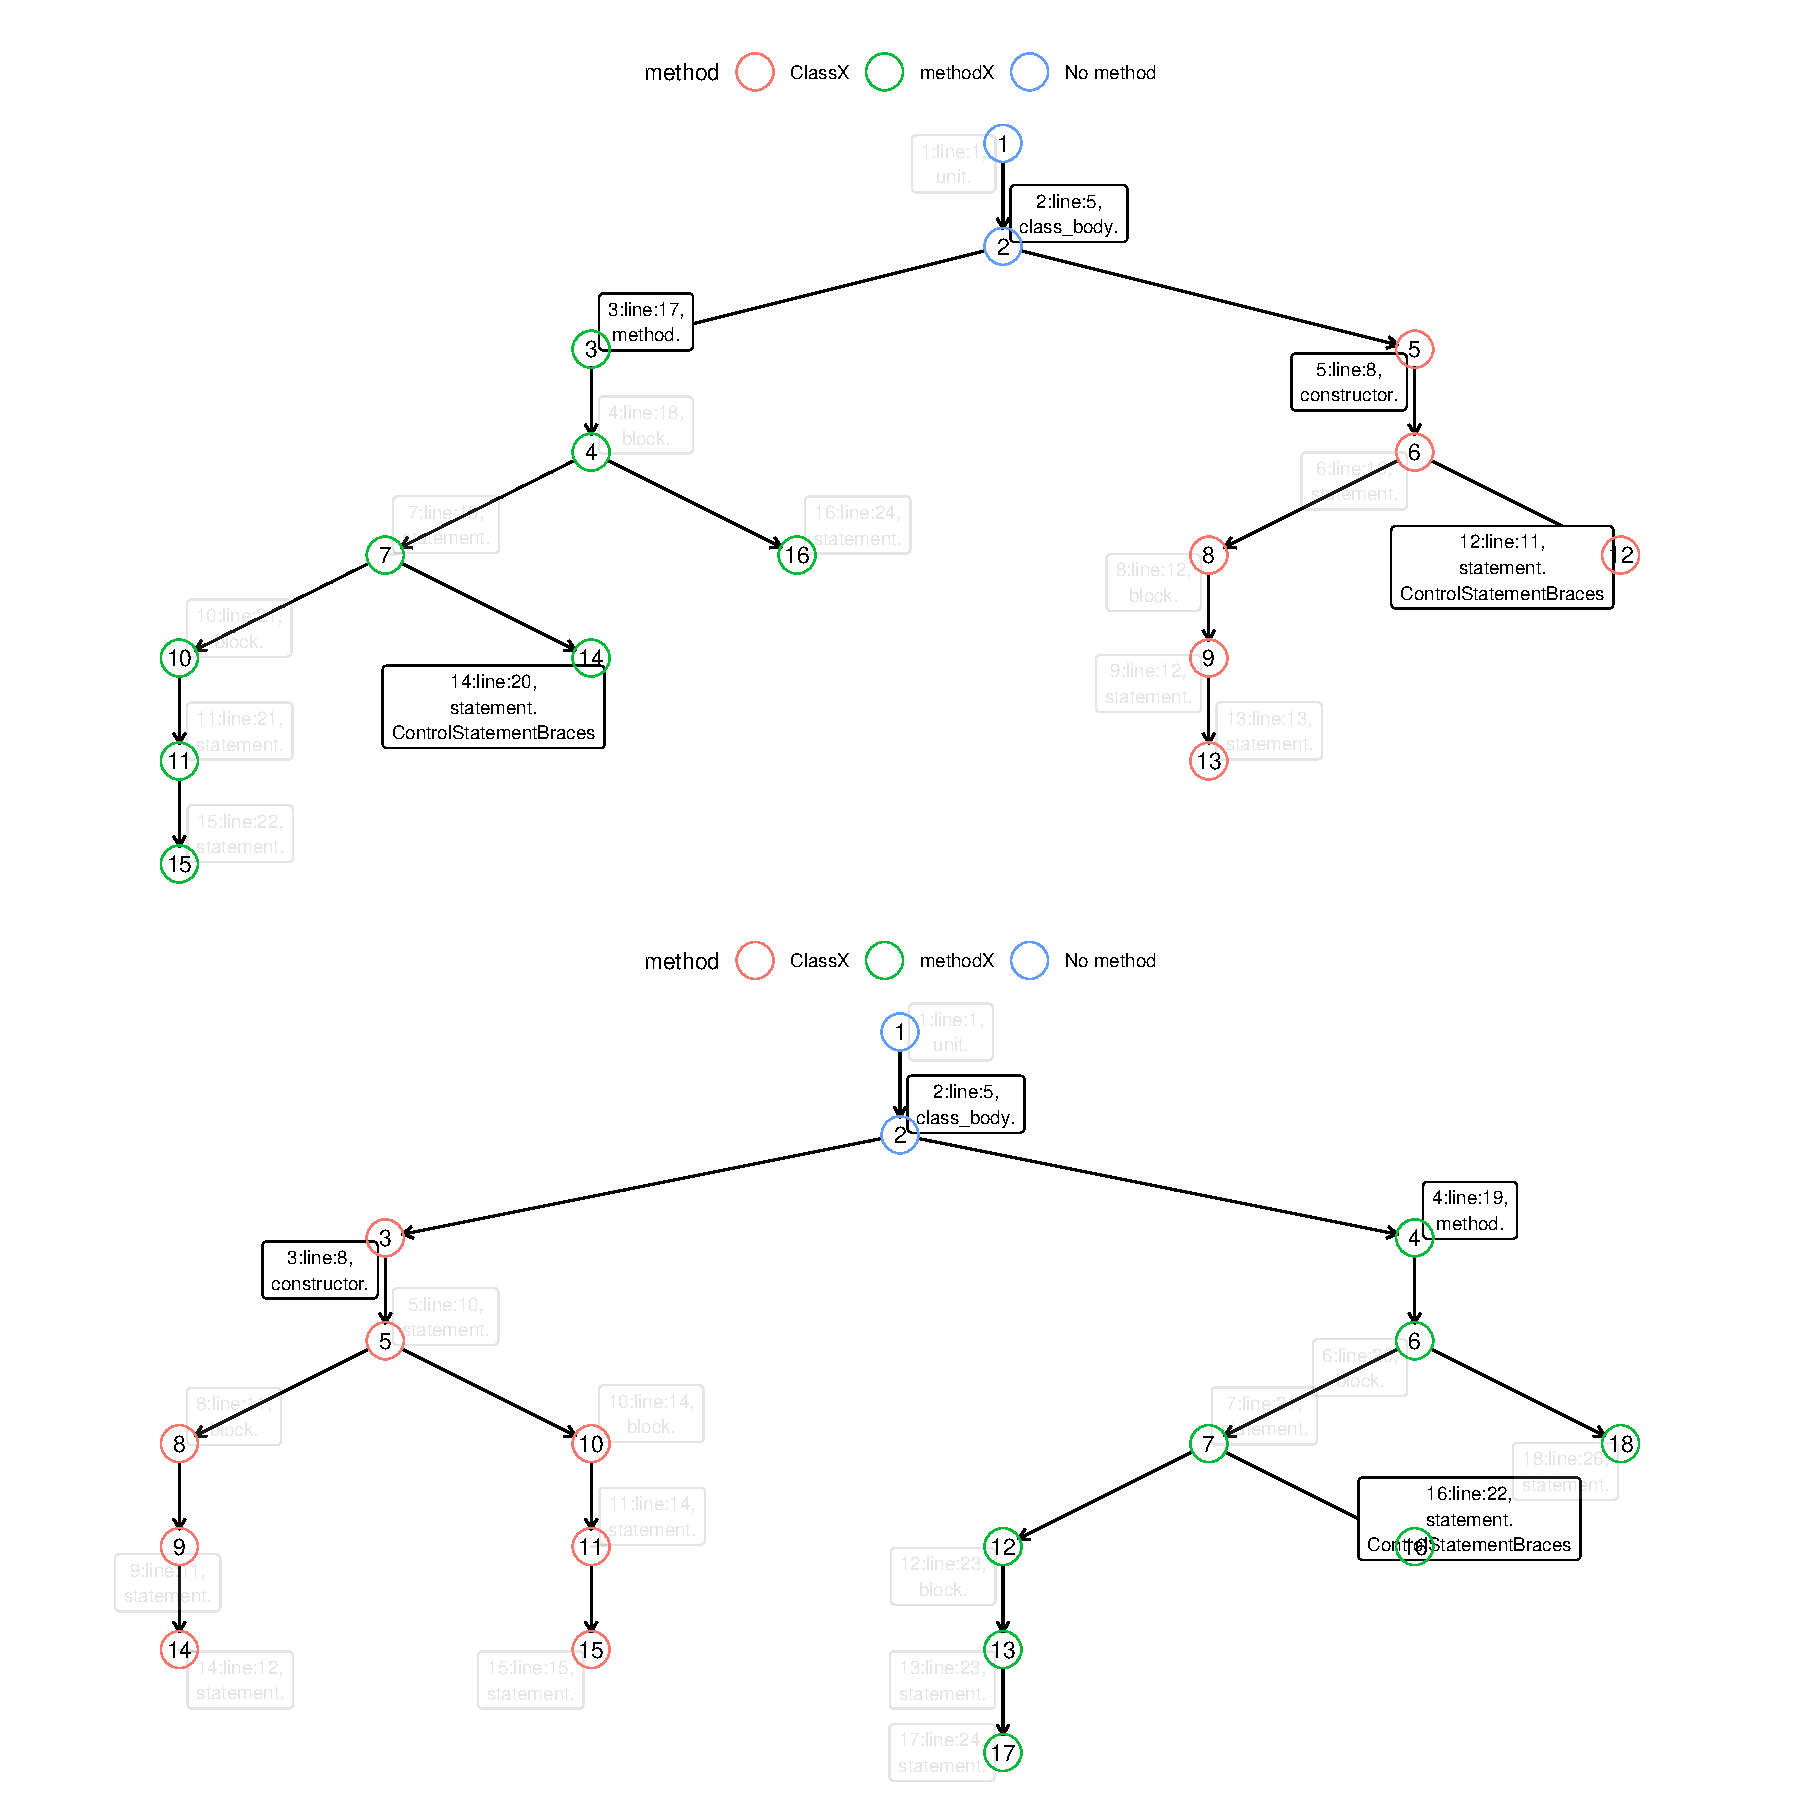
\includegraphics[width=1\linewidth]{report_files/figure-latex/unnamed-chunk-5-1} \caption{Abstract Syntax Trees. New and old versions, with alerts \label{AST_compare_id_alerts}}\label{fig:unnamed-chunk-5}
\end{figure}

\normalsize

\subsection{Map new lines to old lines}\label{map}

For each difference stated in the output of \textit{git diff} (the
sections of the diff file starting with ``@@'\,'), there is an
indication of the number of lines removed from the old version and the
number of lines added to the new one. The line in which the lines are
removed from the old version and the line at which the lines are added
are indicated too. By using this information we create a mapping from
the lines in the old version to the equivalent lines in the new version.
For the new and old versions presented in Section \ref{source_used}, the
relation is shown in Table \ref{table_map}
\footnote{The mapping shown begins at line 5 in order to save space, since lines 1-4 in the old version map to lines 1-4 in the new version.}.

\small

\begin{table}[H]

\caption{\label{tab:showing map }Relation between lines of the old version and lines of the new version\label{table_map}}
\centering
\resizebox{\linewidth}{!}{
\begin{tabular}[t]{l|l|l|l|l|l|l|l|l|l|l|l|l|l|l|l|l|l|l|l|l|l|l|l|l|l|l|l}
\hline
1 & 2 & 3- & -6 & 7 & 8 & \textcolor{white}{7} & 9 & 10 & \textcolor{white}{10} & 11 & \textcolor{white}{12} & 12 & 14 & 13 & \textcolor{white}{16} & 15 & 16 & 17- & -19 & 20 & 21 & 23 & 22 & \textcolor{white}{25} & 24 & 25 & 26\\
\hline
1 & 2 & 3- & -6 & 7 & 8 & 9 & \textcolor{white}{8} & 10 & 11 & 12 & 13 & 14 & \textcolor{white}{14} & 15 & 16 & 17 & 18 & 19- & -21 & 22 & 23 & \textcolor{white}{23} & 24 & 25 & 26 & 27 & 28\\
\hline
\end{tabular}}
\end{table}

\normalsize

\subsection{Calculate features for each pair of new and old alert}

For the proposed example, we calculate features for \(2 \cdot 1 = 2\)
combinations of new and old alerts, since we have 2 old alerts and 1 new
alert. Table \ref{combination} shows the combinations for which features
are calculated.

\small

\begin{table}[H]

\caption{\label{tab:unnamed-chunk-6}Combinations of new and old alerts for which the features must be calculated \label{combination}}
\centering
\begin{tabular}[t]{r|l|r|l}
\hline
Begin Line Old & Rule Old & Begin Line New & Rule New\\
\hline
11 & ControlStatementBraces & 22 & ControlStatementBraces\\
\hline
20 & ControlStatementBraces & 22 & ControlStatementBraces\\
\hline
\end{tabular}
\end{table}

\normalsize

\vspace{16pt}

For each alert, PMD Source Code Analyzer returns the following
attributes:

\vspace{16pt}

We propose the following features to calculate for each combination:

\textbf{Same Rule}: a Boolean indicator that tells if the alerts are of
the same type;

\textbf{Same Group ID}: a Boolean indicator that tells if the alerts are
equivalent in terms of begin line and end line, considering the mapping
described in Section \ref{map}. For each combination, Table
\ref{same_group} shows the begin line in the old version, the
corresponding begin line in the new version, and the begin line in the
new
version\footnote{We suppress the end lines because for all alerts in the 
example the begin lines and the end lines are the same}. The alert that
begins in line 20 of the old version corresponds to the alert that
begins in line 22 of the new version. So, for this combination ``Same
group'\,' feature is true. For the other combination, it is false.

\small

\begin{table}[H]

\caption{\label{tab:unnamed-chunk-7}Same group feature \label{same_group}}
\centering
\resizebox{\linewidth}{!}{
\begin{tabular}[t]{r|l|r|r|l|l}
\hline
Begin Line Old & Rule Old & \makecell[l]{Corresponding line\\ in new version} & Begin Line New & Rule New & Same group\\
\hline
11 & ControlStatementBraces & 12 & 22 & ControlStatementBraces & FALSE\\
\hline
20 & ControlStatementBraces & 22 & 22 & ControlStatementBraces & TRUE\\
\hline
\end{tabular}}
\end{table}

\normalsize

\noindent \textbf{Same Method Group ID}: a Boolean indicator that tells
if the alerts belong to methods that are in the same group in the sense
of the
\texttt{Same\ Group\ ID\textquotesingle{}\textquotesingle{}\ feature\ we\ described\ above.\ First,\ we\ find\ each\ alert\textquotesingle{}s\ method\ following\ the\ path\ from\ the\ alert\textquotesingle{}s\ \ node\ to\ the\ root.\ The\ first\ node\ of\ the\ kind}method'\,'
or ``constructor'\,' found in this path defines the alert's method.
Considering the proposed example, Figure \ref{path_node_to_root_1} shows
the AST for the first combination of alerts (see Table
\ref{combination}).

In this combination, the method of the old alert is in node 5 of the
left tree and the method for the new alert is in node 4 of the right
tree. Table \ref{tab_same_method} shows that the begin and end lines of
the method in the old version do not correspond to the lines in the new
version. The correspondence uses the mapping defined in Section
\ref{map}. For this combination, the ``Same Method Group ID'\,' feature
is FALSE.

\small

\begin{figure}[H]
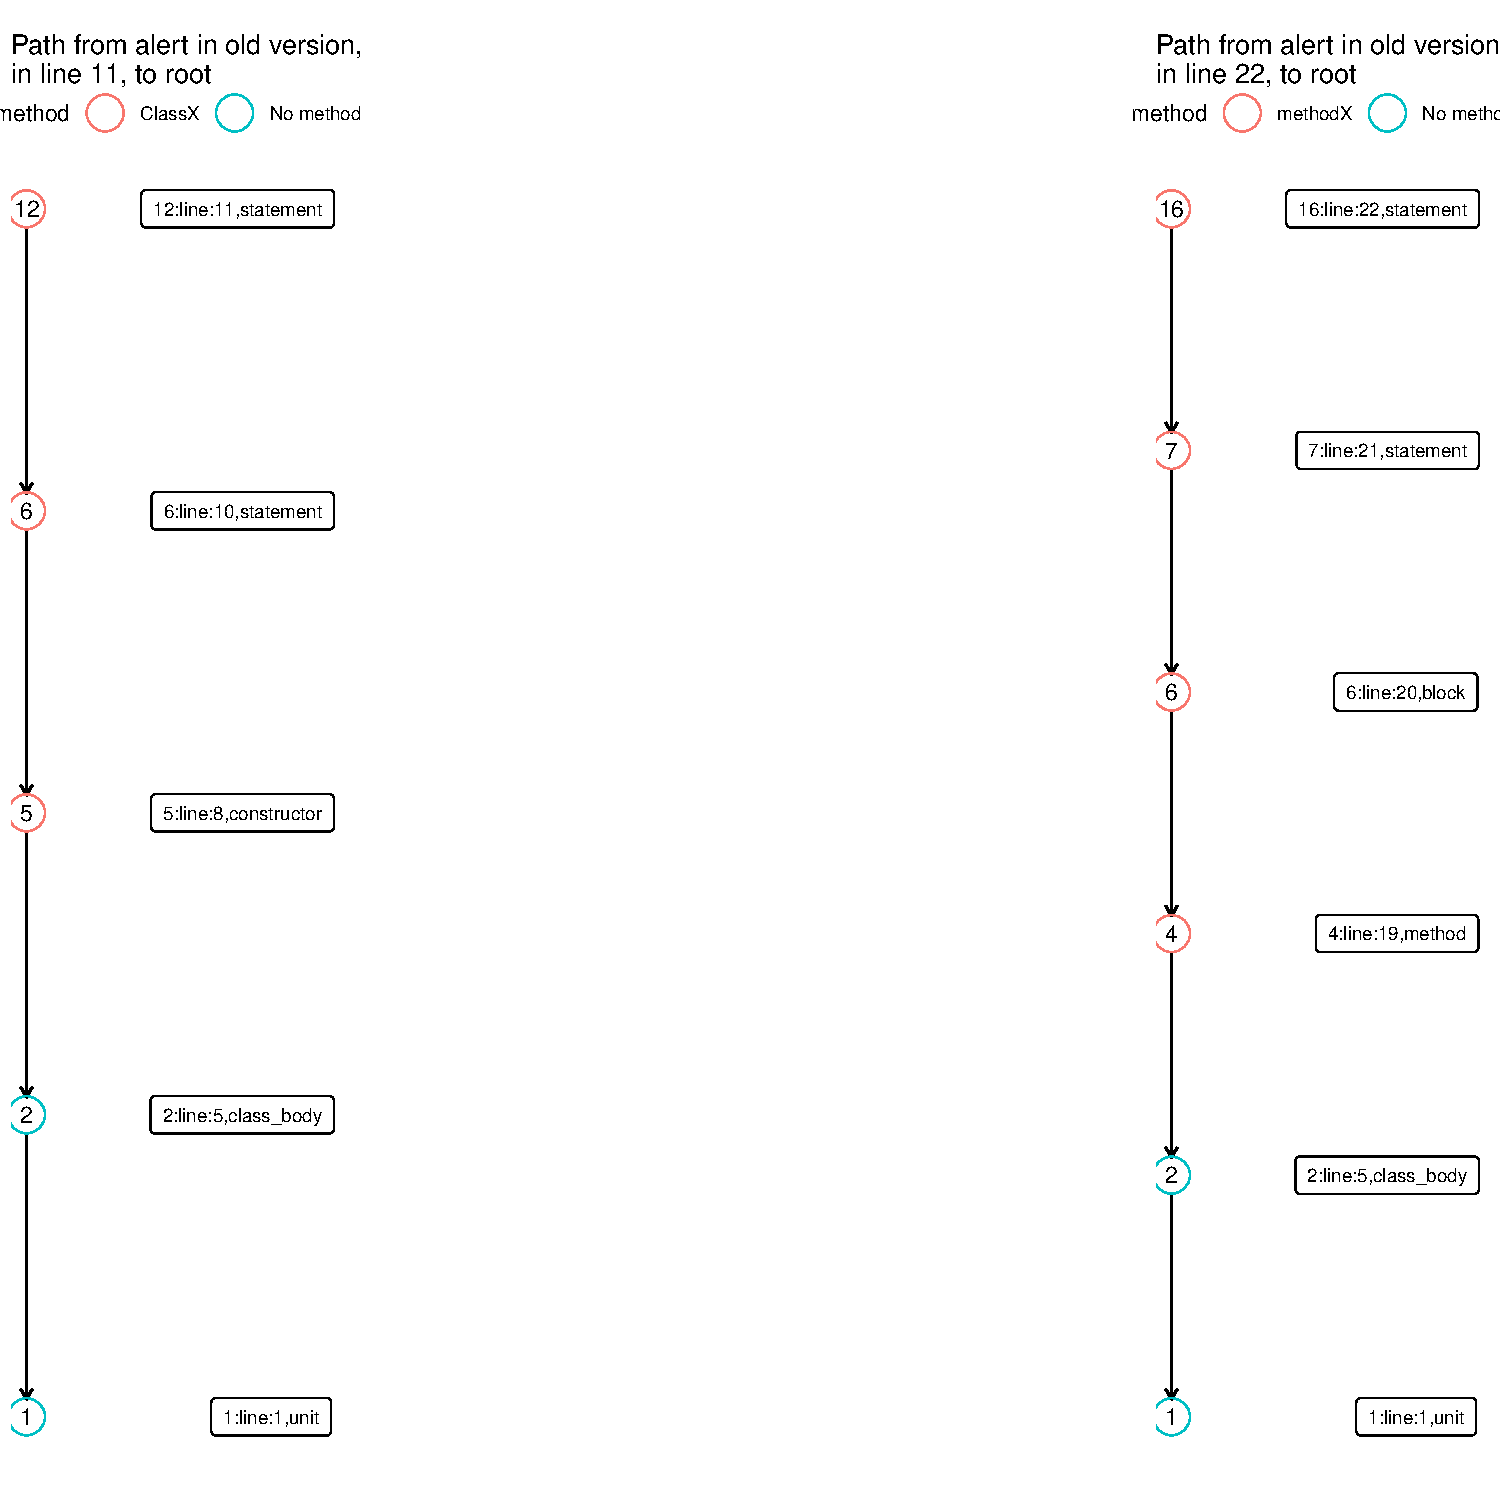
\includegraphics[width=1\linewidth]{report_files/figure-latex/unnamed-chunk-8-1} \caption{Abstract Syntax Tree. Nodes with the same number are equivalent \label{path_node_to_root_1}}\label{fig:unnamed-chunk-8}
\end{figure}

\normalsize

\small

\begin{table}[H]

\caption{\label{tab:unnamed-chunk-9}Defining if Same Method Group ID \label{tab_same_method}}
\centering
\begin{tabular}[t]{l|r|r|r}
\hline
- & Old version & \makecell[l]{Corresponding line\\in the new version} & New version\\
\hline
Begin line & 8 & 8 & 19\\
\hline
End line & 15 & 17 & 27\\
\hline
\end{tabular}
\end{table}

\normalsize

Figure \ref{path_node_to_root_2} shows the ASTs for the second
combination of alerts (see Table \ref{combination}). In this combination
the method of the old alert is in node 3 of the left tree and the method
for the new alert is in node 4 of the right tree. Table
\ref{tab_same_method_2} shows that the begin and end lines of the method
in the old version do correspond to the lines in the new version. The
correspondence uses the map defined in Section \ref{map}. For this
combination, the ``Same Method Group ID'\,' feature is TRUE.

\begin{figure}[H]
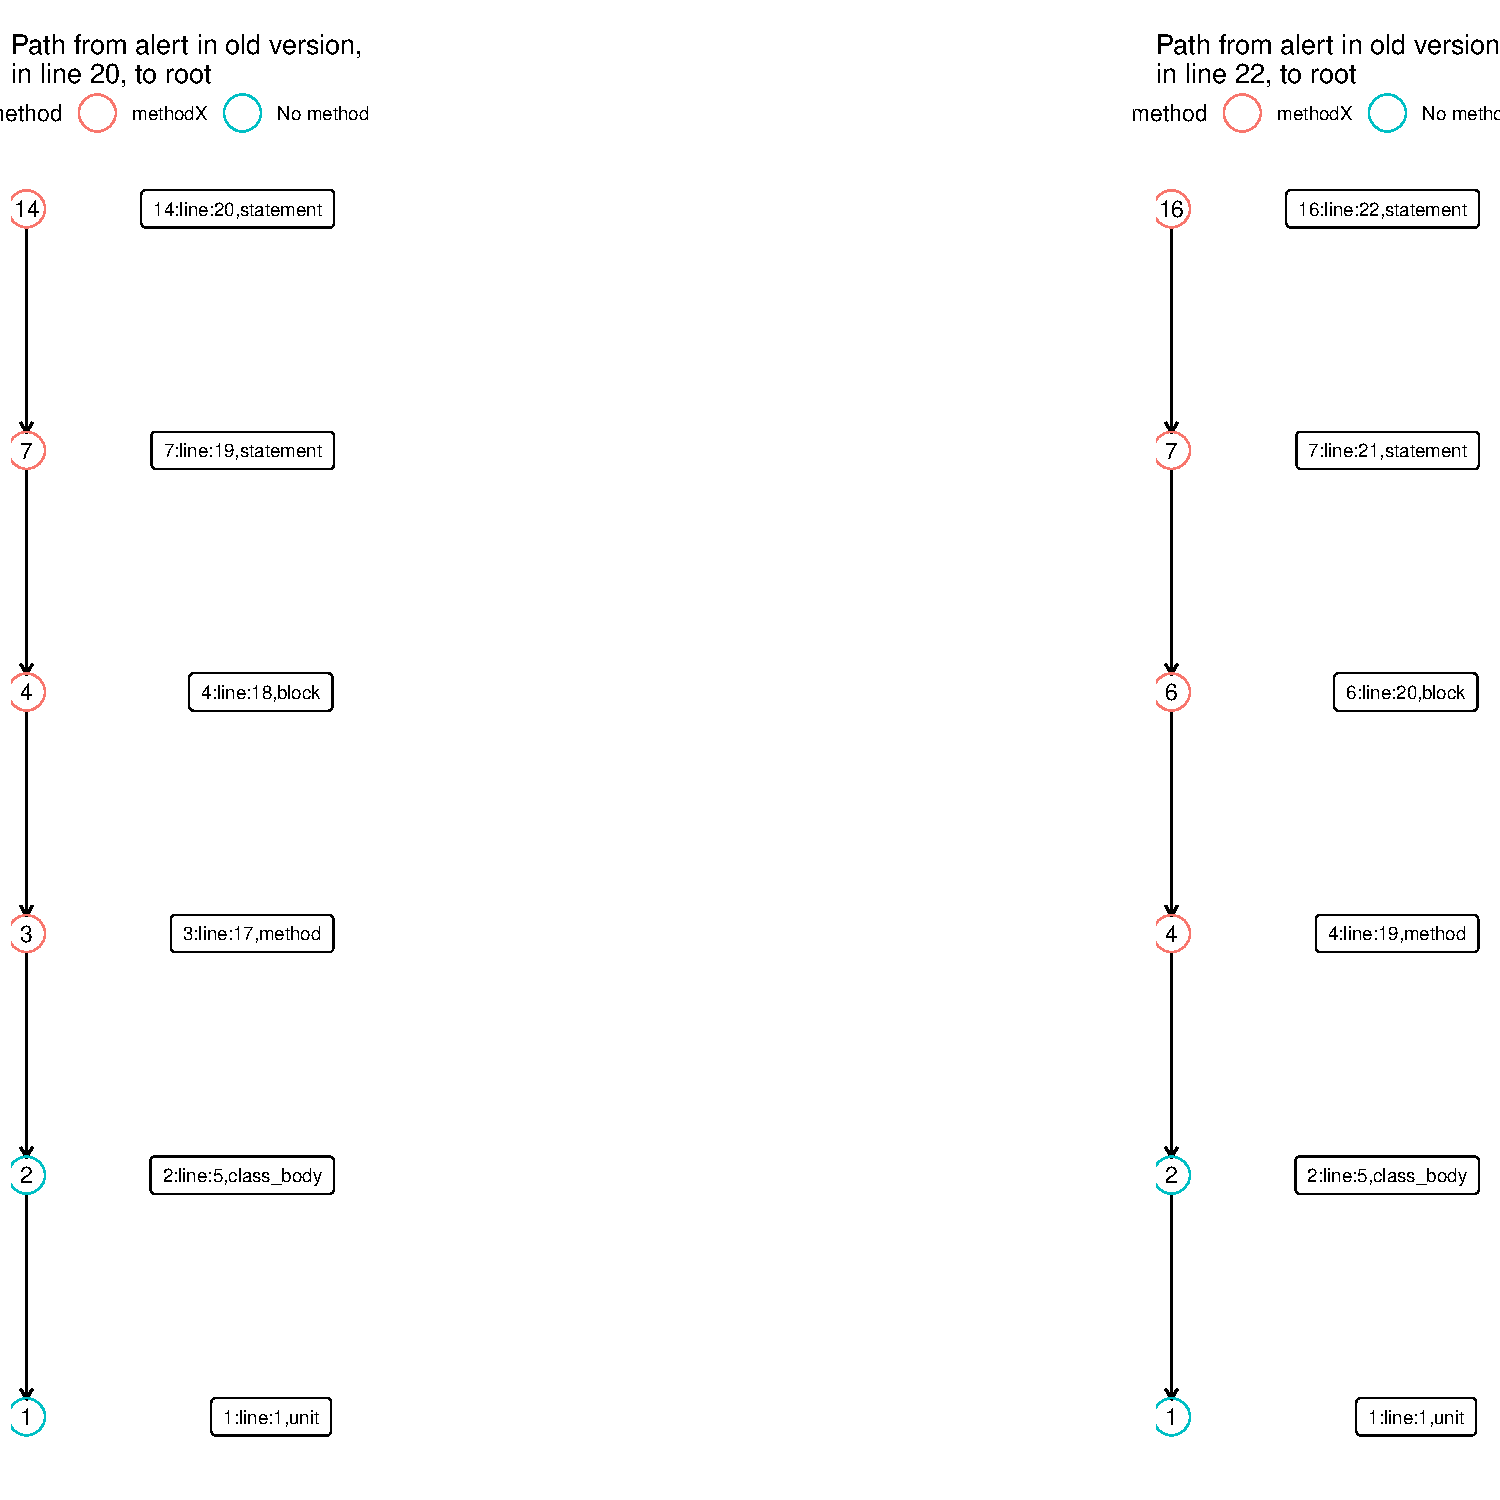
\includegraphics[width=1\linewidth]{report_files/figure-latex/unnamed-chunk-10-1} \caption{Abstract Syntax Tree. Nodes with the same number are equivalent \label{path_node_to_root_2}}\label{fig:unnamed-chunk-10}
\end{figure}

\begin{table}[H]
\caption{\label{tab:unnamed-chunk-11}Defining if Same Method Group ID \label{tab_same_method_2}}
\centering
\begin{tabular}[t]{l|r|r|r}
\hline
- & Old version & \makecell[l]{Corresponding line\\in the new version} & New version\\
\hline
Begin line & 17 & 19 & 19\\
\hline
End line & 25 & 27 & 27\\
\hline
\end{tabular}
\end{table}

\noindent \textbf{Same Method Name}: a Boolean indicator that tells if
the alerts were found in a method with the same name. The methods for
the alerts are found as for the ``Same Method Group ID'\,'. However,
instead of the corresponding lines, this feature evaluates the name of
the methods. If the method related to the old alert and the method
related to the new alert have the same name (even if the begin and end
lines are not corresponding), then this feature is set to TRUE.

\noindent \textbf{Same Block}: a Boolean indicator that shows if the
alerts belong to the same block. The blocks are defined in a similar way
as described above, following the path from the node where each alert is
towards the root until we find a
\texttt{block\textquotesingle{}\textquotesingle{},}method'`, or
\texttt{constructor\textquotesingle{}\textquotesingle{}\ node.\ Then,\ the\ begin\ and\ end\ lines\ \ of\ the\ old\ alert\ and\ the\ corresponding\ lines\ in\ the\ new\ version\ are\ compared\ with\ the\ begin\ and\ end\ lines\ of\ the\ new\ alert,\ as\ for\ the}Same
Method Group ID''.

\noindent \textbf{Same Code}: for this feature we compare the source
code that is contained in the nodes related to the alerts. The
comparison is performed by lexicographically comparing the textual
version of the source code residing within the lines and columns ranges
(begin and end) of the alerts.

\noindent \textbf{Same Method Code}: for this feature we compare the
source code of the methods related to the alerts. The methods related to
the alerts are found the way we described for the ``Same Method Group
ID'\,' above.

\noindent \textbf{Line distance}: the distance between the
\texttt{mean\ line\textquotesingle{}\textquotesingle{}\ (\textbackslash{}(\textbackslash{}frac\{beginline\ +\ endline\}\{2\}\textbackslash{}))\ of\ the\ new\ alert\ and\ the}corresponding
mean line'\,' of the old alert. Table \ref{tab_line_distance} shows the
line distance for the combinations of new and old alerts in the example
we are following.

\small

\begin{table}[H]
\caption{\label{tab:unnamed-chunk-12}Line distance feature \label{tab_line_distance}}
\centering
\resizebox{\linewidth}{!}{
\begin{tabular}[t]{r|r|r|r|r|r|l|r|r}
\hline
\makecell[l]{Begin Line\\Old} & \makecell[l]{End Line\\Old} & \makecell[l]{Corresponding\\begin line\\in new version} & \makecell[l]{Corresponding\\end line\\in new version} & \makecell[l]{Begin Line\\New} & \makecell[l]{End Line\\New} & \makecell[l]{Corresponding\\mean line} & \makecell[l]{Mean line of\\new alert} & Line distance\\
\hline
11 & 11 & 12 & 12 & 22 & 22 & (12 + 12) / 2 = 12 & 22 & 10\\
\hline
20 & 20 & 22 & 22 & 22 & 22 & (22 + 22) / 2 = 22 & 22 & 0\\
\hline
\end{tabular}}
\end{table}

\normalsize

Table \ref{table_features} shows the features calculated for the
combinations of new and old alerts in our example.

\small

\begin{table}[H]

\caption{\label{tab:unnamed-chunk-13}Resulting features\label{table_features} }
\centering
\begin{tabular}[t]{l|l|l}
\hline
Alert combination & Feature & Value\\
\hline
\rowcolor{gray!6}  \rowcolor{gray!6}   & Same Rule & TRUE\\

 & Same Group ID & FALSE\\

\rowcolor{gray!6}   & Same Method Group ID & FALSE\\

 & Same Method Name & FALSE\\

\rowcolor{gray!6}   & Same Block & FALSE\\

 & Same Code & FALSE\\

\rowcolor{gray!6}   & Same Method Code & FALSE\\

\multirow[t]{-8}{*}{\raggedright\arraybackslash Line (Old version):11, Line (New version):22} & Line Distance & 10.00\\
\cline{1-3}
 & Same Rule & TRUE\\

 & Same Group ID & TRUE\\

\rowcolor{gray!6}   & Same Method Group ID & TRUE\\

 & Same Method Name & TRUE\\

\rowcolor{gray!6}   & Same Block & TRUE\\

 & Same Code & TRUE\\

\rowcolor{gray!6}   & Same Method Code & TRUE\\

\multirow[t]{-8}{*}{\raggedright\arraybackslash Line (Old version):20, Line (New version):22} & Line Distance & 0.00\\
\hline
\end{tabular}
\end{table}

\normalsize

\subsection{Decide if two alerts are the same based on heuristic}\label{heuristic}

With the features at hand, we must decide if each combination of old and
new alerts refers to the same alert. As a starting point, we are using a
rule of thumb (a manually-devised heuristic) to make this decision. A
new and an old alerts are declared the same if any of the following
rules apply.

All the Boolean features are TRUE and \textit{Line Distance} is equal to
0;

\scriptsize

\[
\begin{aligned}
(SameRule \land SameGroupID \land SameMethodGroupID \land \\
SameMethodName \land SameBlock \land SameCode \land \\
SameMethodCode \land LineDistance = 0) \Rightarrow SameAlert
\end{aligned}\]

\normalsize

If \textit{Same Method Code} is TRUE, then we consider it is the same
method, even if the name or the method is not the same. But if the
method code is the same, then the alert code and the kind of the alert
must be the same;

\normalsize

If the kind of alert is the same, and at least one of the features about
the method is TRUE, we consider that the alerts are the same if the line
distance must be less then 5 lines;

\scriptsize

\[
\begin{aligned}
(SameRule \land 
(SameMethodCode \lor SameMethodGroup \lor SameMethodName) \land 
LineDistance < 5) \Rightarrow SameAlert
\end{aligned}\]

\normalsize

Table \ref{table_features_with_decision} shows the resulting features of
the two combinations of alerts in the example we are following and the
final decision if they are the same alert.

\small

\begin{table}[H]

\caption{\label{tab:unnamed-chunk-14}Resulting features\label{table_features_with_decision} }
\centering
\begin{tabular}[t]{l|l|l|l}
\hline
Alert combination & Feature & Featre value & Same alert\\
\hline
\rowcolor{gray!6}  \rowcolor{gray!6}   & Same Rule & TRUE & \\

 & Same Group ID & FALSE & \\

\rowcolor{gray!6}   & Same Method Group ID & FALSE & \\

 & Same Method Name & FALSE & \\

\rowcolor{gray!6}   & Same Block & FALSE & \\

 & Same Code & FALSE & \\

\rowcolor{gray!6}   & Same Method Code & FALSE & \\

\multirow[t]{-8}{*}{\raggedright\arraybackslash Line (Old version):11, Line (New version):22} & Line Distance & 10.00 & \multirow[t]{-8}{*}{\raggedright\arraybackslash FALSE}\\
\cline{1-4}
 & Same Rule & TRUE & \\

 & Same Group ID & TRUE & \\

\rowcolor{gray!6}   & Same Method Group ID & TRUE & \\

 & Same Method Name & TRUE & \\

\rowcolor{gray!6}   & Same Block & TRUE & \\

 & Same Code & TRUE & \\

\rowcolor{gray!6}   & Same Method Code & TRUE & \\

\multirow[t]{-8}{*}{\raggedright\arraybackslash Line (Old version):20, Line (New version):22} & Line Distance & 0.00 & \multirow[t]{-8}{*}{\raggedright\arraybackslash TRUE}\\
\hline
\end{tabular}
\end{table}

\normalsize

\subsection{Classify alerts}\label{heuristic}

Finally we can decide if the alerts in the old version are open or fixed
and if the alerts in the new version are open or new. In our example, we
have two alerts in the old version and they are combined with the alert
in the new version. Table \ref{tab_categorizing_old} shows the two old
alerts combined with the new alert. The first old alert is not
classified as the same as any of new alerts, so is marked as
\textbf{Open}. The second alert is classified as the same as the new
alert, so is declared \textbf{Fixed}.

\small

\begin{table}[H]

\caption{\label{tab:unnamed-chunk-15}Categorizing alerts of the old version \label{tab_categorizing_old} }
\centering
\begin{tabular}[t]{r|r|l|l}
\hline
\makecell[l]{Begin line of the alert\\in the old version} & \makecell[l]{Begin line of the alert\\n the new version which\\is combined to the old alert} & \makecell[l]{Same alert according\\to heuristic,\\ based on features} & Category\\
\hline
\rowcolor{gray!6}  11 & 22 & FALSE & OPEN\\
\cline{1-4}
20 & 22 & TRUE & FIXED\\
\hline
\end{tabular}
\end{table}

\normalsize

Table \ref{tab_categorizing_new} shows the new alert combined with the
two old alerts. The new alert is classified as the same as one of the
old alerts, so is declared Open.

\small

\begin{table}[H]

\caption{\label{tab:unnamed-chunk-16}Categorizing alerts of the old version \label{tab_categorizing_new} }
\centering
\begin{tabular}[t]{r|r|l|l}
\hline
\makecell[l]{Begin line of the alert\\in the new version} & \makecell[l]{Begin line of the alert\\n the old version which\\is combined to the old alert} & \makecell[l]{Same alert according\\to heuristic,\\ based on features} & Category\\
\hline
\rowcolor{gray!6}   & 11 & FALSE & \\

\multirow[t]{-2}{*}{\raggedleft\arraybackslash 22} & 20 & TRUE & \multirow[t]{-2}{*}{\raggedright\arraybackslash OPEN}\\
\hline
\end{tabular}
\end{table}

\normalsize

Table \ref{tab_summary_categories} shows the final categories for the
two alerts in the old version and the alert in the new version.

\small

\begin{table}[H]

\caption{\label{tab:unnamed-chunk-17}Alerts and their categorization\label{tab_summary_categories} }
\centering
\begin{tabular}[t]{l|l}
\hline
Alert & Category\\
\hline
\rowcolor{gray!6}  Alert in the old version, line 11 & FIXED\\
\hline
Alert in the old version, line 20 & OPEN\\
\hline
\rowcolor{gray!6}  Alert in the old version, line 22 & OPEN\\
\hline
\end{tabular}
\end{table}

\normalsize

\section{Comparing new alerts with new SATD comments}\label{results}

In this section, we study the correlation between the creation of new
alerts and the insertion of \textit{Self-Admitted Technical Debt}
comments in a transition between an old and a new version of source
code.

%
% MARCIO: colocar as referências abaixo como referências e não escritas diretamente
% no texto.
%

Potdar and Shihab (2014) discuss that the existence of comments that contain specific patterns may indicate what they call Self-Admitted Technical Debts (SATD). Sierra, Shihab, and Kamei (2019) define Self-Admitted Technical Debt as the event in which the developer consciously introduces debt. According to these work, the developer acknowledges the SATD in the form of comments. Wehaibi (2016) presents some patterns based on the work of Potdar and Shihab (2014). These patterns include, though they are not limited to, ``hack'', ``retarded'', ``remove this code'', ``treat this as a soft error'', ``kludge'', ``fixme'', ``this isn't quite right'', ``fix this crap'', ``abandon all hope'' and ``kaboom''. We used all the terms mentioned by the authors and added other terms that we found in code and which we considered indicators of SATDs. To find these additional terms, we sampled 5,000 comments and looked at them to recognize expressions that we judged as indicators of SATDs. The regular expressions representing these terms are listed in the Appendix.

We selected 32 tagged and released versions of the ArgoUML project. They were released between 2001-04-06 and 2011-12-15. For each pair of sequential versions, we generated the PMD Alerts and categorised them as \textbf{New}, \textbf{Fixed} or \textbf{Open} using the algorithm described in Section \ref{alg}. We want to understand if the number of new alerts, normalized by the magnitude of the change between two versions, is a good proxy for the amount of kludge introduced in the code base. A first approach we try in this preliminary investigation is to measure the correlation between the normalized amount of new alerts and comments indicating SADT. %\textit{Self-Admitted Technical Debt}.

The first plot in Figure \ref{timeseries} shows the number of alerts at the end of each version transition. The second plot shows the number of new and fixed alerts. The third plot shows the number of comments that contain expressions listed in the Section \ref{sec_SATDs}. The fourth plot shows the number of new and fixed comments in each version transition. We classify each comment as \textbf{New}, \textbf{Fixed}, and \textbf{Open} by using the following procedure: if the text in the comment is the same as in the preceding version, the comment is classified as \textbf{Open}; the remaining ones are classified as \textbf{Fixed}, if they are in the old version, or \textbf{New} if appeared in the new version.

\begin{figure}
    \centering
    \resizebox{0.75\linewidth}{!}{
        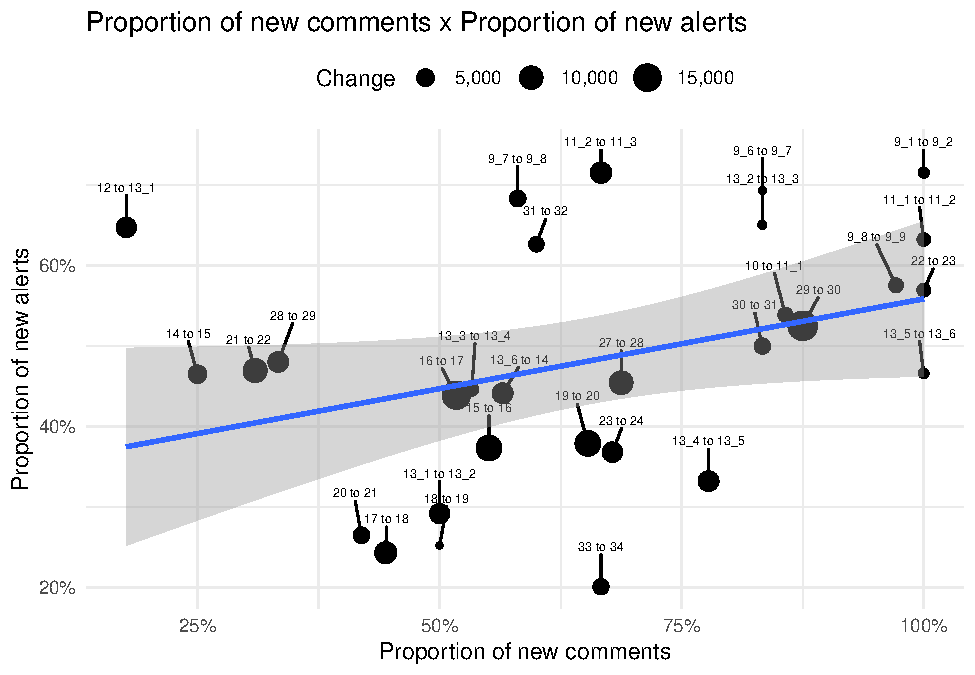
\includegraphics{report_files/figure-latex/unnamed-chunk-21-1.pdf}
    }
    \caption{\label{timeseries}Changes, alerts and comments}
\end{figure}

Hereafter, we analysed the relation between the amount of new alerts and the amount of new comments. The proportion of new alerts and new comments are given by the equations below. We have found that the correlation between the proportion of new alerts and the proportion of new comments is 0.50.

\[NewAlertsProportion = \frac{NewAlerts}{NewAlerts + OldAlerts}\]

\[NewCommentsProportion = \frac{NewComments}{NewComments + OldComments}\]

%
% MARCIO: você não definir OldAlerts. OldAlerts = Open?
%

%
% MARCIO: na seção 3 você menciona uma análise, mas aqui faz outra. Qual é a mais
% correta? Faz sentido fazer as duas? Com certeza não faz sentido ter uma lá e
% outra aqui.
%



Figure \ref{scatter_prop} shows a scatter plot with the relation between the proportion of new alerts and the proportion of new comments. We added a regression line obtained using the following model:

\[ NewCommentsProportion = \alpha + \beta \times NewAlertsProportion \]

The shaded region represents the confidence interval of the prediction of the proportion of alerts given the proportion of comments. As in any linear regression model, the confidence interval is wider in the extremes, since there is uncertainty related to the estimator of intercept \(\hat{\alpha}\) and also to the estimator of the slope of the regression line \(\hat{\beta}\).
   
\begin{figure}
    \centering
    \resizebox{0.75\linewidth}{!}{
    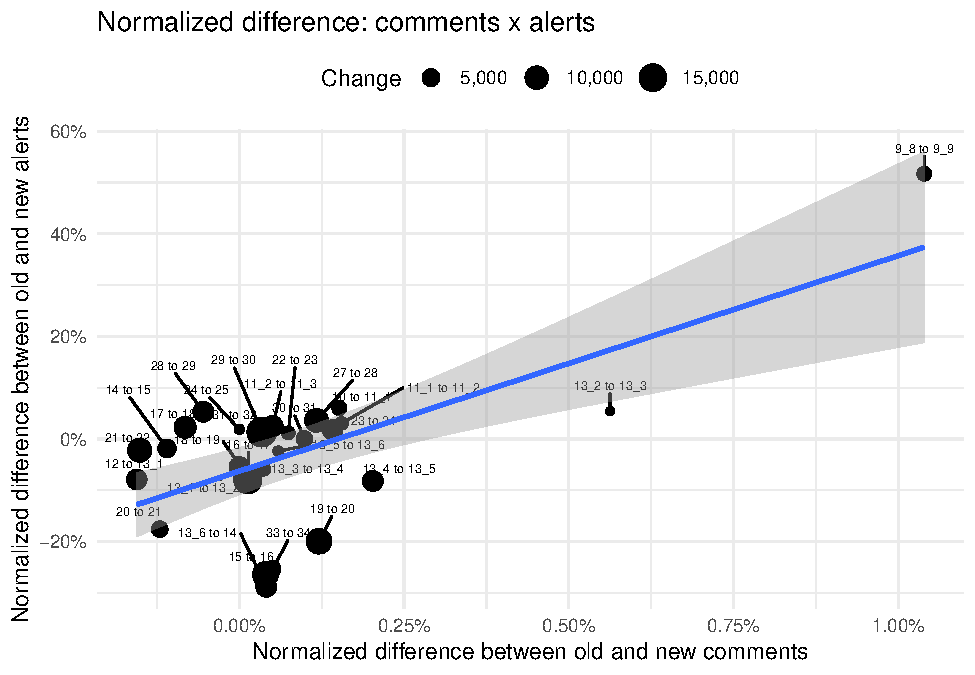
\includegraphics{report_files/figure-latex/unnamed-chunk-23-1.pdf}
    }
    \caption{\label{scatter_prop}Proportion of new alerts x Proportion of
    new comments}
\end{figure}

Next, we evaluated whether the positive correlation we see between the proportion of new comments and the proportion of new alerts was found by chance. Table \ref{tab_reg} shows the results of this regression. The \textit{p-value} of the beta nears zero. This means that it would be very unlikely to get a result as extreme as shown in Figure \ref{scatter_prop} if there wasn't a linear relation between new alerts proportion and new comments proportion. The estimation for \(\beta\) is 0.57, meaning that for each additional 1 pp in the proportion of new alerts we observe, on average, an additional 0.53 pp in the proportion of new comments. The \(R^2\) is 0.25, so we could say that 25\% of the variability in the proportion of new comments is explained by the variation in the proportion of new alerts.

%
% MARCIO: o que é o pp?
%

%
% MARCIO: R2 = 25% é bem ruim. Quanto tempo você levaria para fazer a mesma 
% análise em um segundo projeto?
%

%
% MARCIO: acima "an additional 0.53 pp" seria "an additional 0.57 pp", certo?
%

%
% MARCIO: tem como fazer uma análise qualitativa dos quatro principais outliers?
% o que aconteceu nestas versões?
%

\begin{table}[h!]
\caption{\label{tab:unnamed-chunk-25}\label{tab_reg} Regression: comments on alerts}
\centering
\begin{tabular}[t]{l|rcr}
\hline
 & Beta & 95\% Conf. Interval & p-value\\
\hline
(Intercept) & 0.33 & 0.13, 0.52 & 0.002\\
%\hline
New Alerts Proportion & 0.57 & 0.20, 0.95 & 0.004\\
\hline
%\multicolumn{4}{l}{\textsuperscript{1} CI = Confidence Interval}\\
\end{tabular}
\end{table}

In the next steps, we can refine the way we select the SATD comments. There are papers that use more sophisticated schemes to identify them, using Natural Language Processing, for instance. Following these steps maybe we will be able to get more certainty about the relation between alerts and SATD comments. Maybe we will be able to explain a greater part of the variability in the proportion of new SATD comments.

%
% MARCIO: que papers são estes? Tem referências?
%


% =========================================================
%
% PMD SOURCE CODE ANALYZER
%
% =========================================================

\section*{Appendix: regular expressions used to find SATDs}
\label{sec_SATDs}

\small
\begin{longtable}{r|l}
\hline
\# & Expression\\
\hline
\endfirsthead

\multicolumn{2}{@{}l}{\textit{(continued)}}\\
\hline
\# & Expression\\
\hline
\endhead

1 & (:?doesn't|does not) take into account\\
%\hline
2 & (:?don't|do not) understand\\
%\hline
3 & (:?it|this) (?:is|seems) ?[[:alnum:][:space:]]* a part implementation\\
%\hline
4 & (:?it|this) (?:is|seems) ambiguous\\
%\hline
5 & (:?it|this) ?[[:alnum:][:space:]]* should be\\
%\hline
6 & (:?it|this) ?[[:alnum:][:space:]]* should not\\
%\hline
7 & (:?it|this) ?[[:alnum:][:space:]]* shouldn't\\
%\hline
8 & (:?it|this) is never executed\\
%\hline
9 & (:?it|this) is planned to refactor\\
%\hline
10 & (:?it|this) should ?[[:alnum:][:space:]]* be ?[[:alnum:][:space:]]* the other way round\\
%\hline
11 & (:?it|this) should ?[[:alnum:][:space:]]* be extended\\
%\hline
12 & (:?it|this) should ?[[:alnum:][:space:]]* be using\\
%\hline
13 & (:?this|the|it) ?[[:alnum:][:space:]]* contains a ?[[:alnum:][:space:]]* error\\
%\hline
14 & (?:the|it|this) ?[[:alnum:][:space:]]* only works\\
%\hline
15 & (?:this|it) ?.* does not work\\
%\hline
16 & (?:this|it)?[[:alnum:][:space:]]* is in the wrong place\\
%\hline
17 & (?:todo:|needs-more-work:)[ ]*check\\
%\hline
18 & (?:todo:|needs-more-work:)[ ]*complete this\\
%\hline
19 & (?:todo:|needs-more-work:)[ ]*constraints\\
%\hline
20 & (?:todo:|needs-more-work:)[ ]*document\\
%\hline
21 & (?:todo:|needs-more-work:)[ ]*find a way to\\
%\hline
22 & (?:todo:|needs-more-work:)[ ]*review\\
%\hline
23 & (?:todo:|needs-more-work:)[ ]*verify\\
%\hline
24 & (?:todo:|needs-more-work:)[ ]*what\textbackslash{}?\\
%\hline
25 & (?:todo|needs-more-work): ?[[:alnum:][:space:]]* algorithm\\
%\hline
26 & (?:todo|needs-more-work): ?[[:alnum:][:space:]]* in some cases\\
%\hline
27 & (?:todo|needs-more-work): ?[[:alnum:][:space:]]* incomplete\\
%\hline
28 & (?:todo|needs-more-work): ?[[:alnum:][:space:]]* not ?[[:alnum:][:space:]]* completely\\
%\hline
29 & (?:todo|needs-more-work): ?[[:alnum:][:space:]]* this does\\
%\hline
30 & (?:todo|needs-more-work): ?[[:alnum:][:space:]]* unfinished\\
%\hline
31 & (?:todo|needs-more-work):[ ]*add\\
%\hline
32 & (?:todo|needs-more-work):[ ]*assumes\\
%\hline
33 & (?:todo|needs-more-work):[ ]*constructors\\
%\hline
34 & (?:todo|needs-more-work):[ ]*define\\
%\hline
35 & (?:todo|needs-more-work):[ ]*disable\\
%\hline
36 & (?:todo|needs-more-work):[ ]*fix\\
%\hline
37 & (?:todo|needs-more-work):[ ]*handle\\
%\hline
38 & (?:todo|needs-more-work):[ ]*improve\\
%\hline
39 & (?:todo|needs-more-work):[ ]*make\\
%\hline
40 & (?:todo|needs-more-work):[ ]*move\\
%\hline
41 & (?:todo|needs-more-work):[ ]*not implemented\\
%\hline
42 & (?:todo|needs-more-work):[ ]*provide\\
%\hline
43 & (?:todo|needs-more-work):[ ]*remove\\
%\hline
44 & (?:todo|needs-more-work):[ ]*replace\\
%\hline
45 & (?:todo|needs-more-work):[ ]*should\\
%\hline
46 & (?:todo|needs-more-work):[ ]*split\\
%\hline
47 & (?:todo|needs-more-work):[ ]*this ?[[:alnum:][:space:]]* needs\\
%\hline
48 & (?:todo|needs-more-work):[ ]*this ?[[:alnum:][:space:]]* should\\
%\hline
49 & (?:todo|needs-more-work):[ ]*treat\\
%\hline
50 & (?:todo|needs-more-work):[ ]*use\\
%\hline
51 & (?:todo|needs-more-work):[ ]*we ?[[:alnum:][:space:]]* need\\
%\hline
52 & (?:todo|needs-more-work):[ ]*what\textbackslash{}?\\
%\hline
53 & (?:todo|needs-more-work):[ ]*why\\
%\hline
54 & [do not|don't] ?[[:alnum:][:space:]]* understand the code\\
%\hline
55 & \textbackslash{}:\textbackslash{}-\textbackslash{}(\\
%\hline
56 & a ?[[:alnum:][:space:]]* better way of doing this would\\
%\hline
57 & a better implementation would be\\
%\hline
58 & abandon all hope\\
%\hline
59 & always check for\\
%\hline
60 & at a loss\\
%\hline
61 & at the moment\\
%\hline
62 & awkward\\
%\hline
63 & bad smell\\
%\hline
64 & bail out\\
%\hline
65 & barf\\
%\hline
66 & brute force\\
%\hline
67 & buggy\\
%\hline
68 & can we remove\\
%\hline
69 & cause for issue\\
%\hline
70 & causes issue\\
%\hline
71 & causes? ?[[:alnum:][:space:]]* errors?\\
%\hline
72 & certainly buggy\\
%\hline
73 & check that this is correct\\
%\hline
74 & crap\\
%\hline
75 & crappy\\
%\hline
76 & do not use this\\
%\hline
77 & do we ?[[:alnum:][:space:]]* need ?[[:alnum:][:space:]]* this\\
%\hline
78 & does not handle\\
%\hline
79 & does not work\\
%\hline
80 & does this help\\
%\hline
81 & don't think so\\
%\hline
82 & don't use this\\
%\hline
83 & double counted\\
%\hline
84 & doubt that this would work\\
%\hline
85 & dummy implementation\\
%\hline
86 & enhance so that\\
%\hline
87 & explain that this ?[[:alnum:][:space:]]* works also\\
%\hline
88 & fix this\\
%\hline
89 & fix this crap\\
%\hline
90 & fixme\\
%\hline
91 & for a next refactoring\\
%\hline
92 & fragile\\
%\hline
93 & get rid of this\\
%\hline
94 & give up and go away\\
%\hline
95 & good enough\\
%\hline
96 & hack\\
%\hline
97 & hacky\\
%\hline
98 & hang our heads in shame\\
%\hline
99 & hardcoded\\
%\hline
100 & hardwired\\
%\hline
101 & hope everything will work\\
%\hline
102 & hopefully\\
%\hline
103 & horrible\\
%\hline
104 & how can this possibly be\\
%\hline
105 & how come this happens\\
%\hline
106 & how to avoid\\
%\hline
107 & i'd suggest that\\
%\hline
108 & i [do not|don't] know\\
%\hline
109 & i [do not|don't] see ?[[:alnum:][:space:]]* reason for\\
%\hline
110 & i don't know\\
%\hline
111 & in the future\\
%\hline
112 & inconsistency\\
%\hline
113 & is (:?it|this) possible\\
%\hline
114 & is (?:it|this|the) ?[[:alnum:][:space:]]* still useful\\
%\hline
115 & is (?:this|it) ?[[:alnum:][:space:]]* correct\\
%\hline
116 & is ?[[:alnum:][:space:]]* the right thing here\\
%\hline
117 & is done twice\\
%\hline
118 & is it a bug\\
%\hline
119 & is not so beautiful\\
%\hline
120 & is problematic\\
%\hline
121 & is this .*needed\\
%\hline
122 & is this a good way ?[[:alnum:][:space:]]*\textbackslash{}?\\
%\hline
123 & is this line really safe\\
%\hline
124 & is this next line safe\\
%\hline
125 & it does not work yet\\
%\hline
126 & it doesn't work yet\\
%\hline
127 & it is planned to refactor\\
%\hline
128 & it is unclear to me\\
%\hline
129 & it works,? but\\
%\hline
130 & it would be ?[[:alnum:][:space:]]* more efficient to\\
%\hline
131 & it would be better to\\
%\hline
132 & just a guess\\
%\hline
133 & just abandon it\\
%\hline
134 & kaboom\\
%\hline
135 & kludge\\
%\hline
136 & less elegant ?[[:alnum:][:space:]]* that works\\
%\hline
137 & magic numbers?\\
%\hline
138 & make (?:it|this) configurable\\
%\hline
139 & may cause problem\\
%\hline
140 & nasty\\
%\hline
141 & necessary\textbackslash{}?\\
%\hline
142 & necessary\textbackslash{}?\\
%\hline
143 & need to be changed\\
%\hline
144 & need to be reviewed\\
%\hline
145 & need to replace this\\
%\hline
146 & needs to be ?[[:alnum:][:space:]]* after stable release\\
%\hline
147 & needs to be fixed\\
%\hline
148 & needs to be tidied up\\
%\hline
149 & needs to be updated\\
%\hline
150 & needs to be updated\\
%\hline
151 & never get executed\\
%\hline
152 & no point in doing this\\
%\hline
153 & not exact, but close\\
%\hline
154 & not strictly correct\\
%\hline
155 & not sure ?[[:alnum:][:space:]]* (?:this|it) belongs here\\
%\hline
156 & not sure this is ?[[:alnum:][:space:]]* right\\
%\hline
157 & not sure whether this belongs here\\
%\hline
158 & not the right location\\
%\hline
159 & nuke\\
%\hline
160 & once we go ?[[:alnum:][:space:]]* we won't need this\\
%\hline
161 & ouch\\
%\hline
162 & pending\\
%\hline
163 & please explain this\\
%\hline
164 & potential ?[[:alnum:][:space:]]* issue\\
%\hline
165 & probably a bug\\
%\hline
166 & problematic\\
%\hline
167 & prolly a bug\\
%\hline
168 & prove that this works\\
%\hline
169 & purists would\\
%\hline
170 & really should be\\
%\hline
171 & really should be\\
%\hline
172 & remove me before production\\
%\hline
173 & remove one of them\\
%\hline
174 & remove this before production\\
%\hline
175 & remove this code\\
%\hline
176 & replace by ?[[:alnum:][:space:]]* elegant\\
%\hline
177 & retarded\\
%\hline
178 & risk of this blowing up\\
%\hline
179 & shall not be\\
%\hline
180 & shame\\
%\hline
181 & should match ?[[:alnum:][:space:]]* uml\\
%\hline
182 & should not be using ?[[:alnum:][:space:]]* here\\
%\hline
183 & should there really be ?[[:alnum:][:space:]]* \textbackslash{}?\\
%\hline
184 & shouldn't we ?[[:alnum:][:space:]]* do something ?[[:alnum:][:space:]]* here\\
%\hline
185 & silly\\
%\hline
186 & some fatal error\\
%\hline
187 & something ?[[:alnum:][:space:]]* gone wrong\\
%\hline
188 & something bad happened\\
%\hline
189 & something bad is going on\\
%\hline
190 & something serious is wrong\\
%\hline
191 & strange construction\\
%\hline
192 & stupid\\
%\hline
193 & temporary crutch\\
%\hline
194 & temporary fix\\
%\hline
195 & temporary solution\\
%\hline
196 & test this\\
%\hline
197 & that's for a next refactoring\\
%\hline
198 & the ?[[:alnum:][:space:]]* (?:is|seems) redundant\\
%\hline
199 & there ?[[:alnum:][:space:]]* must be a check\\
%\hline
200 & there ?[[:alnum:][:space:]]* ought to be a check\\
%\hline
201 & there is a problem\\
%\hline
202 & this (?:is|seems) ?[[:alnum:][:space:]]* expensive way to\\
%\hline
203 & this (?:is|seems) a temporary method\\
%\hline
204 & this ?[[:alnum:][:space:]]* (?:is|seems) ?[[:alnum:][:space:]]* redundant\\
%\hline
205 & this can be a mess\\
%\hline
206 & this creates a dependency\\
%\hline
207 & this does exactly the same\\
%\hline
208 & this does not look right\\
%\hline
209 & this doesn't look right\\
%\hline
210 & this error needs to be\\
%\hline
211 & this indicates a ?[[:alnum:][:space:]]* problem\\
%\hline
212 & this is already defined\\
%\hline
213 & this is bs\\
%\hline
214 & this is temporary and will go away\\
%\hline
215 & this is uncool\\
%\hline
216 & this is wrong\\
%\hline
217 & this isn't quite right\\
%\hline
218 & this isn't very solid\\
%\hline
219 & this needs work\\
%\hline
220 & this should use ?[[:alnum:][:space:]]* instead of\\
%\hline
221 & this will ?[[:alnum:][:space:]]* not be perfect\\
%\hline
222 & this will fail\\
%\hline
223 & too primitive\\
%\hline
224 & toss it\\
%\hline
225 & treat .*as a soft error\\
%\hline
226 & trial and error\\
%\hline
227 & turn off after built\\
%\hline
228 & ugly\\
%\hline
229 & unknown why we ever experience this\\
%\hline
230 & untested\\
%\hline
231 & until code is reviewed\\
%\hline
232 & unused?\\
%\hline
233 & wasteful\\
%\hline
234 & we ?[[:alnum:][:space:]]* (?:don't|do not) need (?:it|this) any more\\
%\hline
235 & we ?[[:alnum:][:space:]]* do not want\\
%\hline
236 & we ?[[:alnum:][:space:]]* don't want\\
%\hline
237 & we can remove\\
%\hline
238 & we need a better\\
%\hline
239 & we presume\\
%\hline
240 & we should not need this\\
%\hline
241 & we shouldn't need this\\
%\hline
242 & what (?:shall|should) we do here\\
%\hline
243 & what do we want to use .*\textbackslash{}?\\
%\hline
244 & what if we need to .*\textbackslash{}?\\
%\hline
245 & what is this trying to do\textbackslash{}?\\
%\hline
246 & why (?:is|are) ?[[:alnum:][:space:]]* being ignored\\
%\hline
247 & why ?[[:alnum:][:space:]]* continue here as if nothing has gone wrong\textbackslash{}?\\
%\hline
248 & why aren't we ?[[:alnum:][:space:]]* \textbackslash{}?\\
%\hline
249 & why is this code commented\\
%\hline
250 & why isn't this done\\
%\hline
251 & why there is not test\\
%\hline
252 & workaround\\
%\hline
253 & workaround for bug\\
%\hline
254 & would be better here\\
%\hline
255 & you can be unhappy now\\
%\hline
256 & yuck\\
\hline
\end{longtable}



\normalsize


% =========================================================
%
% PMD SOURCE CODE ANALYZER
%
% =========================================================

\section*{References}

\hypertarget{refs}{}
\begin{cslreferences}
\leavevmode\hypertarget{ref-Potdar2014}{}%
Potdar, Aniket, and Emad Shihab. 2014. ``An exploratory study on
self-admitted technical debt.'' \emph{Proceedings - 30th International
Conference on Software Maintenance and Evolution, ICSME 2014}, 91--100.
\url{https://doi.org/10.1109/ICSME.2014.31}.

\leavevmode\hypertarget{ref-Sierra2019}{}%
Sierra, Giancarlo, Emad Shihab, and Yasutaka Kamei. 2019. ``A survey of
self-admitted technical debt.'' Elsevier Inc.
\url{https://doi.org/10.1016/j.jss.2019.02.056}.

\leavevmode\hypertarget{ref-Wehaibi2016}{}%
Wehaibi, Sultan. 2016. ``Satd-Patterns.''
\url{https://github.com/xsultan/satd-patterns}.
\end{cslreferences}

\end{document}
